\PassOptionsToPackage{unicode=true}{hyperref} % options for packages loaded elsewhere
\PassOptionsToPackage{hyphens}{url}
\PassOptionsToPackage{dvipsnames,svgnames*,x11names*}{xcolor}
%
\documentclass[ignorenonframetext,]{beamer}
\usepackage{pgfpages}
\setbeamertemplate{caption}[numbered]
\setbeamertemplate{caption label separator}{: }
\setbeamercolor{caption name}{fg=normal text.fg}
\beamertemplatenavigationsymbolsempty
% Prevent slide breaks in the middle of a paragraph:
\widowpenalties 1 10000
\raggedbottom
\setbeamertemplate{part page}{
\centering
\begin{beamercolorbox}[sep=16pt,center]{part title}
  \usebeamerfont{part title}\insertpart\par
\end{beamercolorbox}
}
\setbeamertemplate{section page}{
\centering
\begin{beamercolorbox}[sep=12pt,center]{part title}
  \usebeamerfont{section title}\insertsection\par
\end{beamercolorbox}
}
\setbeamertemplate{subsection page}{
\centering
\begin{beamercolorbox}[sep=8pt,center]{part title}
  \usebeamerfont{subsection title}\insertsubsection\par
\end{beamercolorbox}
}
\AtBeginPart{
  \frame{\partpage}
}
\AtBeginSection{
  \ifbibliography
  \else
    \frame{\sectionpage}
  \fi
}
\AtBeginSubsection{
  \frame{\subsectionpage}
}
\usepackage{lmodern}
\usepackage{amssymb,amsmath}
\usepackage{ifxetex,ifluatex}
\usepackage{fixltx2e} % provides \textsubscript
\ifnum 0\ifxetex 1\fi\ifluatex 1\fi=0 % if pdftex
  \usepackage[T1]{fontenc}
  \usepackage[utf8]{inputenc}
  \usepackage{textcomp} % provides euro and other symbols
\else % if luatex or xelatex
  \usepackage{unicode-math}
  \defaultfontfeatures{Ligatures=TeX,Scale=MatchLowercase}
\fi
% use upquote if available, for straight quotes in verbatim environments
\IfFileExists{upquote.sty}{\usepackage{upquote}}{}
% use microtype if available
\IfFileExists{microtype.sty}{%
\usepackage[]{microtype}
\UseMicrotypeSet[protrusion]{basicmath} % disable protrusion for tt fonts
}{}
\IfFileExists{parskip.sty}{%
\usepackage{parskip}
}{% else
\setlength{\parindent}{0pt}
\setlength{\parskip}{6pt plus 2pt minus 1pt}
}
\usepackage{xcolor}
\usepackage{hyperref}
\hypersetup{
            pdftitle={Introduction to Epidemiological and Biostatistical Thinking},
            pdfauthor={Marlena Bannick},
            colorlinks=true,
            linkcolor=Maroon,
            filecolor=Maroon,
            citecolor=Blue,
            urlcolor=blue,
            breaklinks=true}
\urlstyle{same}  % don't use monospace font for urls
\newif\ifbibliography
\usepackage{graphicx,grffile}
\makeatletter
\def\maxwidth{\ifdim\Gin@nat@width>\linewidth\linewidth\else\Gin@nat@width\fi}
\def\maxheight{\ifdim\Gin@nat@height>\textheight\textheight\else\Gin@nat@height\fi}
\makeatother
% Scale images if necessary, so that they will not overflow the page
% margins by default, and it is still possible to overwrite the defaults
% using explicit options in \includegraphics[width, height, ...]{}
\setkeys{Gin}{width=\maxwidth,height=\maxheight,keepaspectratio}
\setlength{\emergencystretch}{3em}  % prevent overfull lines
\providecommand{\tightlist}{%
  \setlength{\itemsep}{0pt}\setlength{\parskip}{0pt}}
\setcounter{secnumdepth}{0}

% set default figure placement to htbp
\makeatletter
\def\fps@figure{htbp}
\makeatother

\usetheme[
  outer/progressbar=foot,
  outer/numbering=none,
  sectionpage=progressbar,
  progressbar=frametitle
]{metropolis}
\definecolor{Purple}{HTML}{4b2e83}
\definecolor{Black}{HTML}{000000}
\definecolor{Orange}{HTML}{1C608A}
\definecolor{White}{HTML}{FFFFFF}
\definecolor{Gold}{HTML}{746643}
\definecolor{LightGold}{HTML}{D2C7AC}
\setbeamercolor{alerted text}{fg=Gold}
\setbeamercolor{frametitle}{bg=Purple, fg=LightGold}
\setbeamercolor{title}{fg=Gold}
\setbeamercolor{subtitle}{fg=Black}
\setbeamercolor{normal text}{fg=Black}
\setbeamercolor{background canvas}{bg=White}
\setbeamertemplate{itemize items}{$-$}

\title{Introduction to Epidemiological and Biostatistical Thinking}
\providecommand{\subtitle}[1]{}
\subtitle{UW Neurology Fellowship}
\author{Marlena Bannick}
\providecommand{\institute}[1]{}
\institute{PhD Student, University of Washington Dept. of Biostatistics\\
Researcher, Institute for Health Metrics and Evaluation}
\date{7/23/2020}

\begin{document}
\frame{\titlepage}

\begin{frame}{Goal}
\protect\hypertarget{goal}{}

Introduce you to epidemiological thinking and key (bio)statistical
concepts that you can use to critically interpret scientific studies in
health and medicine.

\end{frame}

\begin{frame}{Learning Objectives (1/2)}
\protect\hypertarget{learning-objectives-12}{}

\begin{enumerate}
\tightlist
\item
  \textbf{Basics}. Identify key elements of an epidemiological study and
  how they relate to the scientific question
\item
  \textbf{Study Design}. Recognize the basic types of epidemiological
  study design and identify when each design is appropriate for the
  scientific question
\item
  \textbf{Bias}. Recognize sources of bias in study designs or
  measurements and understand how they might affect your ability to
  answer the scientific question
\end{enumerate}

\end{frame}

\begin{frame}{Learning Objectives (2/2)}
\protect\hypertarget{learning-objectives-22}{}

\begin{enumerate}
\setcounter{enumi}{3}
\tightlist
\item
  \textbf{Modeling}. Understand how you can formulate your understanding
  about a data generating process, assumptions, and a hypothesis to test
  in a statistical model
\item
  \textbf{Inference}. Recognize the distinction between an effect size,
  a confidence interval, and a p-value as they relate to parameters that
  are estimated in a statistical model
\end{enumerate}

TODO -- talk about \(\beta\) inference in the example

\end{frame}

\begin{frame}{Further Study}
\protect\hypertarget{further-study}{}

This lecture and follow-up discussion will be a very brief introduction,
with some material borrowed from the following texts. These are good
introduction texts to epidemiology and biostatistics:


\includegraphics[width=0.3\textwidth,height=\textheight]{../media/gordis.jpg}

\includegraphics[width=0.3\textwidth,height=\textheight]{../media/hebel-carter.jpg}

\end{frame}

\begin{frame}{Basics}
\protect\hypertarget{basics}{}

A epidemiological study should be generated by a \emph{scientific
question of interest}. Broadly, you can think of these scientific
questions falling into two main categories:

\begin{itemize}
\tightlist
\item
  \textbf{Descriptive}: What is the incidence rate of ischemic stroke
  (IS) in women aged 45 - 60 years old?
\item
  \textbf{Inferential}: What is the effect of an experimental treatment
  on mortality following ischemic stroke in women aged 45 - 60?
\end{itemize}

From a statistical point of view it is not a clean distinction because
you still use statistical tools to \emph{infer} the incidence rate for a
descriptive study.

\end{frame}

\begin{frame}{Basics: Terminology}
\protect\hypertarget{basics-terminology}{}

The questions \emph{who, what, where, when} have never been more
important than in the context of epidemiology!

Having a well-defined scientific question means having clear answers for
the following components:

\begin{itemize}
\tightlist
\item
  \textbf{population}: Who is the group being studied? Study populations
  should be representative of the target population that the study
  results will be generalized to.
\item
  \textbf{exposure}: What is the group in study exposed to that you want
  to measure the effect of, and over what period of time?
\item
  \textbf{outcome}: What outcome is being studied (either in relation to
  the exposure or on its own) and over what period of time?
\end{itemize}

\end{frame}

\begin{frame}{Basics: Measures}
\protect\hypertarget{basics-measures}{}

Once you've defined your target exposure, outcome, and population that
makes up your scientific questions, understanding \textbf{measurement}
of the outcomes is of utmost importance.

Some common outcome measurements in the context of health sciences are

\begin{itemize}
\tightlist
\item
  \textbf{prevalence}: proportion of a population with an outcome
\item
  \textbf{incidence}: rate of getting the outcome among individuals in a
  population that did not already have the outcome (``risk'')
\item
  \textbf{remission}: rate of returning to be outcome-free among those
  that had the outcome
\item
  \textbf{odds}: \(\frac{p}{1 - p}\) where \(p\) is a proportion
\end{itemize}

\emph{Think about denominators!}

\end{frame}

\begin{frame}{Basics: Measures for Comparisons}
\protect\hypertarget{basics-measures-for-comparisons}{}

Common measures of comparison between two exposure groups include
functions of the measures we just discussed:

\begin{itemize}
\tightlist
\item
  \textbf{relative risk} or \textbf{risk difference}: comparing
  incidence of an outcome between two groups as a difference or a ratio
\item
  \textbf{odds ratio}: comparing odds of an outcome between two groups
  as a ratio
\end{itemize}

\end{frame}

\begin{frame}{Basics: 2x2 Tables}
\protect\hypertarget{basics-2x2-tables}{}

With a binary exposure and a binary outcome, the results of a study will
look something like this 2x2 table:

\begin{table}[!h]

\caption{\label{tab:table3}Example 2x2 Table}
\centering
\begin{tabular}{l|l|l}
\hline
 & Outcome & No Outcome\\
\hline
Exposed & a & c\\
\hline
Unexposed & b & d\\
\hline
\end{tabular}
\end{table}

But there are \emph{so many ways} to obtain that 2x2 table, so it is
imperative to understand the study design behind the data!

Understanding study design will make it clear \textbf{what are the valid
analyses} that can be performed on the data in that table.

\end{frame}

\begin{frame}{Basics: Example}
\protect\hypertarget{basics-example}{}

What are the exposure, outcome, and population for the following
scientific question?

\textbf{What is the effect of an experimental treatment on mortality
following ischemic stroke in women age 45 - 60?}

\begin{itemize}
\tightlist
\item
  Population:
\item
  Exposure:
\item
  Outcome:
\end{itemize}

\end{frame}

\begin{frame}{Basics: Example}
\protect\hypertarget{basics-example-1}{}

What are the exposure, outcome, and population for the following
scientific question?

\textbf{What is the effect of an experimental treatment on mortality
following ischemic stroke in women age 45 - 60?}

\begin{itemize}
\tightlist
\item
  Population: \textbf{women age 45-60 who have had ischemic stroke}
\item
  Exposure: \textbf{experimental treatment}
\item
  Outcome: \textbf{death from ischemic stroke}
\end{itemize}

How would you make these questions more precise?

\end{frame}

\begin{frame}{Study Design: Types}
\protect\hypertarget{study-design-types}{}

Starting with what is typically considered the studies that will provide
the ``strongest'' evidence of a \emph{causal} relationship between an
exposure and an outcome:

Experimental Designs

\begin{itemize}
\tightlist
\item
  Randomized controlled trials
\end{itemize}

Observational Designs

\begin{itemize}
\tightlist
\item
  Cohort studies
\item
  Case control studies
\item
  Cross-sectional studies
\item
  Case reports
\end{itemize}

\end{frame}

\begin{frame}{Study Design: Randomized Controlled Trials}
\protect\hypertarget{study-design-randomized-controlled-trials}{}

An experimental setting in which participants are enrolled and then
\emph{randomly} assigned to a treatment or a control and followed up
over time to record outcomes.

\begin{itemize}
\tightlist
\item
  Ideal for inferring causal relationships because there are no
  significant differences between treatment and control groups, both in
  terms of factors we can measure and factors we cannot measure (more
  later with confounding)
\item
  They are expensive, time consuming, and not always feasible or ethical
  (think smoking)
\end{itemize}

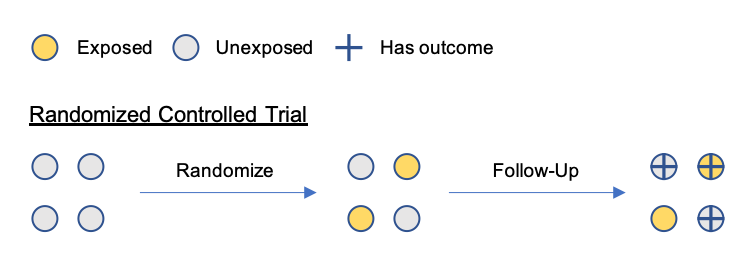
\includegraphics[width=0.85\textwidth,height=\textheight]{../media/study-design-rct.png}

\end{frame}

\begin{frame}{Study Design: Cohort Study}
\protect\hypertarget{study-design-cohort-study}{}

An observational design where participants are selected based on their
exposure status and followed up to record outcomes at designated time
points.

\begin{itemize}
\tightlist
\item
  Similar to a randomized controlled trial with one key difference: the
  exposures are not randomized! You may only \textbf{observe what is
  already happening}.
\end{itemize}

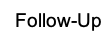
\includegraphics[width=0.85\textwidth,height=\textheight]{../media/study-design-cohort.png}

\end{frame}

\begin{frame}{Study Design: Case-Control Study}
\protect\hypertarget{study-design-case-control-study}{}

An observational design where participants are selected based on their
outcome status and we inquire about exposure in the past. Think of it as
the opposite of a cohort study, looking back in time.

\begin{itemize}
\tightlist
\item
  May be subject to biases like \emph{recall bias} (more later)
\item
  The artificial distribution of cases and controls means you cannot
  naively compute ``prevalence'' of the outcome or ``relative risk''
\end{itemize}

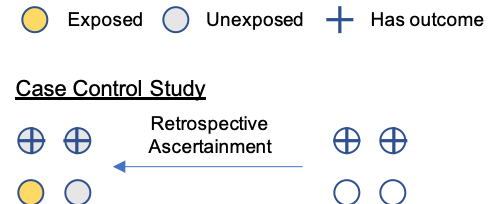
\includegraphics{../media/study-design-cc.png}

\end{frame}

\begin{frame}{Study Design: Cross-Sectional Study}
\protect\hypertarget{study-design-cross-sectional-study}{}

An observational design where you measure exposure and outcome of
participants at the same point in time (no temporal element).

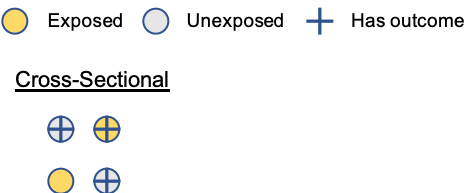
\includegraphics{../media/study-design-cross.png}

\end{frame}

\begin{frame}{Study Design: Case Report}
\protect\hypertarget{study-design-case-report}{}

An observational design where you report on the outcome status of one or
a handful of interesting cases. ``Anecdotal'' evidence.

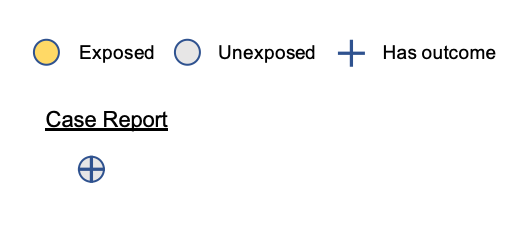
\includegraphics{../media/study-design-case.png}

\end{frame}

\begin{frame}{Study Design: Example}
\protect\hypertarget{study-design-example}{}

Recall our example: \textbf{What is the effect of an experimental
treatment on mortality following ischemic stroke in women age 45 - 60?}

Which of the following designs would you prefer to answer this
scientific question and why?

\begin{itemize}
\tightlist
\item
  Randomized controlled trial
\item
  Cohort study
\item
  Case control study
\item
  Cross-sectional
\item
  Case report
\end{itemize}

\end{frame}

\begin{frame}{Biases: Taxonomy}
\protect\hypertarget{biases-taxonomy}{}

Biases in the epidemiological context are any factors in your study that
\textbf{prevent you from being able to answer your precise scientific
question}.

Biases may result from systematically flawed measurements of the
outcome, the exposure, or the population, categorized generally as:

\begin{itemize}
\tightlist
\item
  \textbf{\textcolor{red}{selection biases}}: biases that are a function
  of the sampling or selection of participants for the study
  -\textgreater{} cannot generalize to target population
\item
  \textbf{\textcolor{blue}{information biases}}: biases that are a
  function of how the measurements on participants are taken
\end{itemize}

Some study designs may avoid certain types of bias, but it is crucial to
always be on the lookout for sneaky biases when designing, analyzing, or
reading a study.

\end{frame}

\begin{frame}{Biases: Examples}
\protect\hypertarget{biases-examples}{}

Examples of biases include:

\begin{itemize}
\tightlist
\item
  \textbf{\textcolor{red}{Loss to follow-up bias}}: participants leave
  the study in such a way that it distorts the relationship between the
  exposure and outcome
\item
  \textbf{\textcolor{blue}{Confounding bias}}: the relationship between
  exposure and outcome among those in your study is \emph{confounded} by
  other variables (more later)
\item
  \textbf{\textcolor{blue}{Recall bias}}: individuals are being asked
  about exposures or outcomes that they do not remember correctly
\item
  \textbf{\textcolor{blue}{Social desirability bias}}: individuals are
  not comfortable disclosing their true exposure or outcome status for
  fear of judgement by others
\end{itemize}

This is by no means an exhaustive list. See
\href{https://catalogofbias.org/biases/}{a catalogue of bias} for a
taxonomy and more examples.

\end{frame}

\begin{frame}{Biases: Selection Bias Diagram}
\protect\hypertarget{biases-selection-bias-diagram}{}

An example of selection bias is loss to follow-up. Consider a situation
where

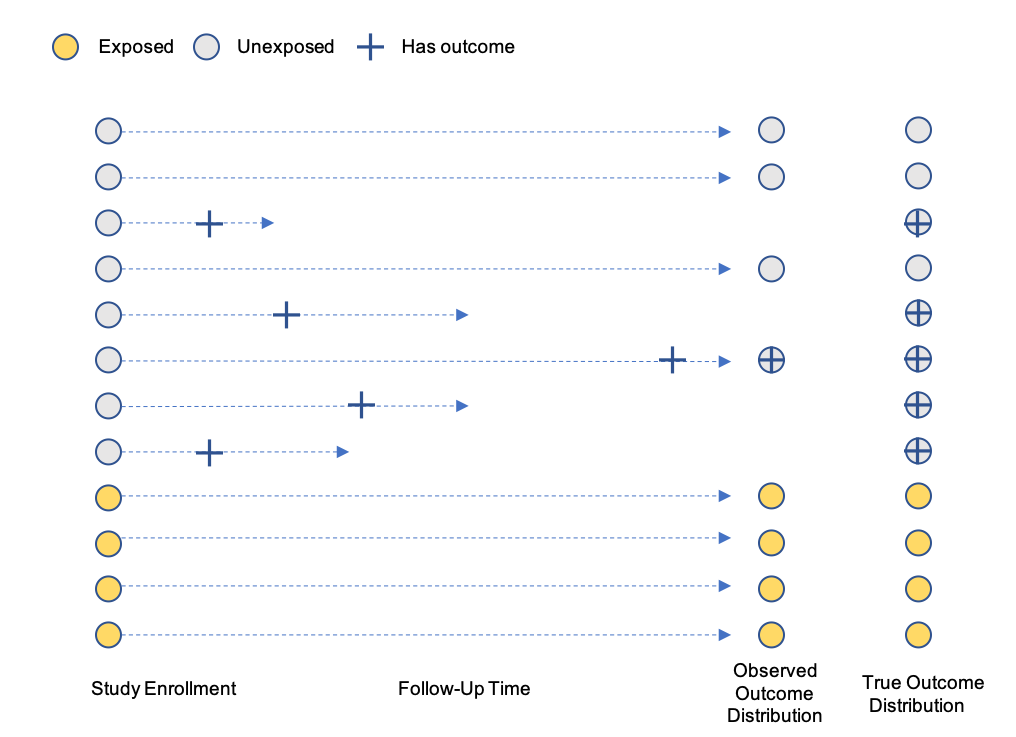
\includegraphics[width=0.75\textwidth,height=\textheight]{../media/loss-to-followup.png}

\end{frame}

\begin{frame}{Biases: Selection Bias Example}
\protect\hypertarget{biases-selection-bias-example}{}

Recall our example inferential question: \textbf{What is the effect of
an experimental treatment on mortality following ischemic stroke in
women age 45 - 60?}

Consider the following sampling strategies:

\begin{enumerate}
\tightlist
\item
  Sample women aged 45 - 60 who have been discharged from the hospital
  following ischemic stroke, randomly assign some to experimental
  treatment.
\item
  Sample women aged 45 - 60 who have been admitted to the hospital for
  ischemic stroke, randomly assign some to experimental treatment.
\end{enumerate}

Which may suffer from selection bias?

\end{frame}

\begin{frame}{Biases: Confounding Diagram}
\protect\hypertarget{biases-confounding-diagram}{}

Confounding occurs when there is a third, measured or unmeasured, factor
\(Z\) that causes the exposure \(X\) and is associated (perhaps
causally) with the outcome \(Y\). If \(X \to Z\), then it is not a
confounder because \(Z\) is \emph{in the causal pathway} between \(X\)
and \(Y\).

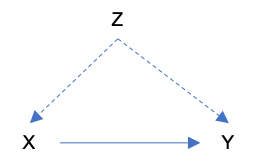
\includegraphics{../media/confounding-basic.png}

If we have \textbf{measured} \(Z\), then there is hope that we can
recover the true relationship between \(X\) and \(Y\). If \(Z\) is
unmeasured (which is often the case), it is much more difficult. In the
case where \(Z\) is measured, there are standard techniques to
``control'' for \(Z\).

\end{frame}

\begin{frame}{Biases: Confounding Example}
\protect\hypertarget{biases-confounding-example}{}

Again, recall our example inferential question: \textbf{What is the
effect of an experimental treatment on mortality following ischemic
stroke in women age 45 - 60?}

What if we do not assign the experimental treatment, but the physician
decides whether or not to administer treatment to the patient?

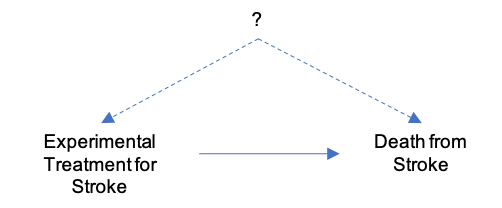
\includegraphics{../media/confounding-example-q.png}

\end{frame}

\begin{frame}{Biases: Confounding and Stratification (1/5)}
\protect\hypertarget{biases-confounding-and-stratification-15}{}

Consider a study where we have an equal number of exposed and unexposed
participants, and we want to follow them over time to observe an
outcome.

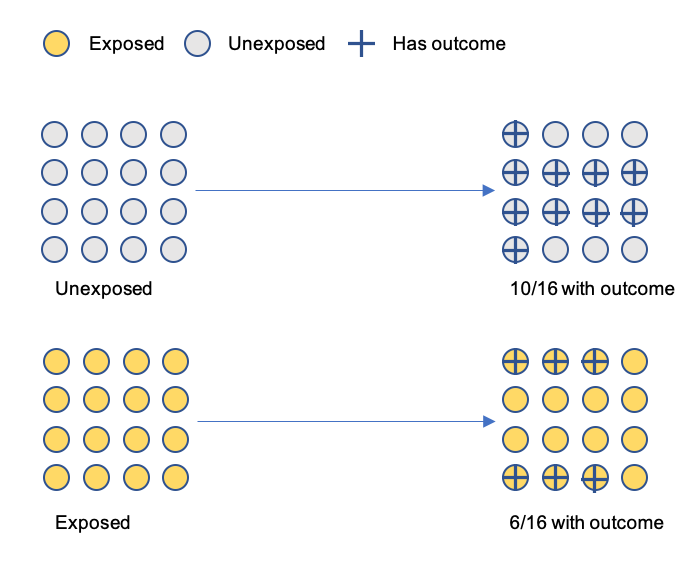
\includegraphics[width=0.75\textwidth,height=\textheight]{../media/confounder-1.png}

\end{frame}

\begin{frame}{Biases: Confounding and Stratification (2/5)}
\protect\hypertarget{biases-confounding-and-stratification-25}{}

If you saw the result below, you would conclude that the exposure is
protective: the proportion of participants with the outcome is much
greater among the unexposed than the exposed.

Confounding occurs when there is a hidden (and hopefully measured!)
factor, indicated by the red outline. The distribution of the hidden
factor differs among the exposed and unexposed, and among those that
have and don't have the outcome.

\end{frame}

\begin{frame}{Biases: Confounding and Stratification (3/5)}
\protect\hypertarget{biases-confounding-and-stratification-35}{}

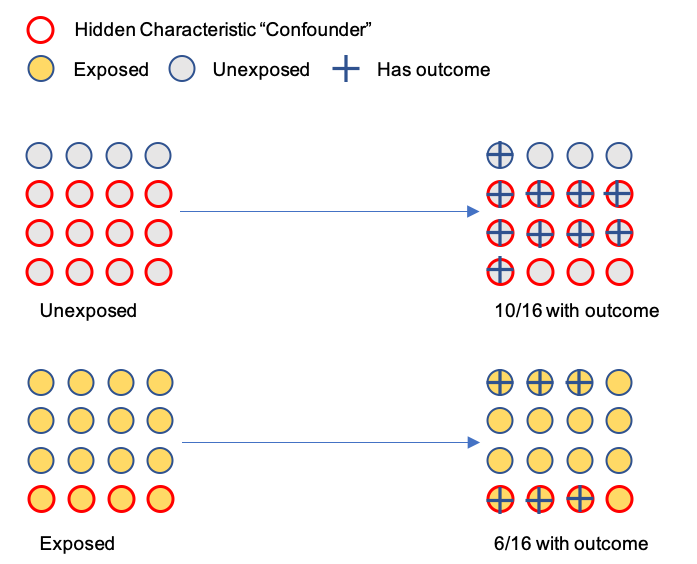
\includegraphics[width=0.75\textwidth,height=\textheight]{../media/confounder-2.png}

\end{frame}

\begin{frame}{Biases: Confounding and Stratification (4/5)}
\protect\hypertarget{biases-confounding-and-stratification-45}{}

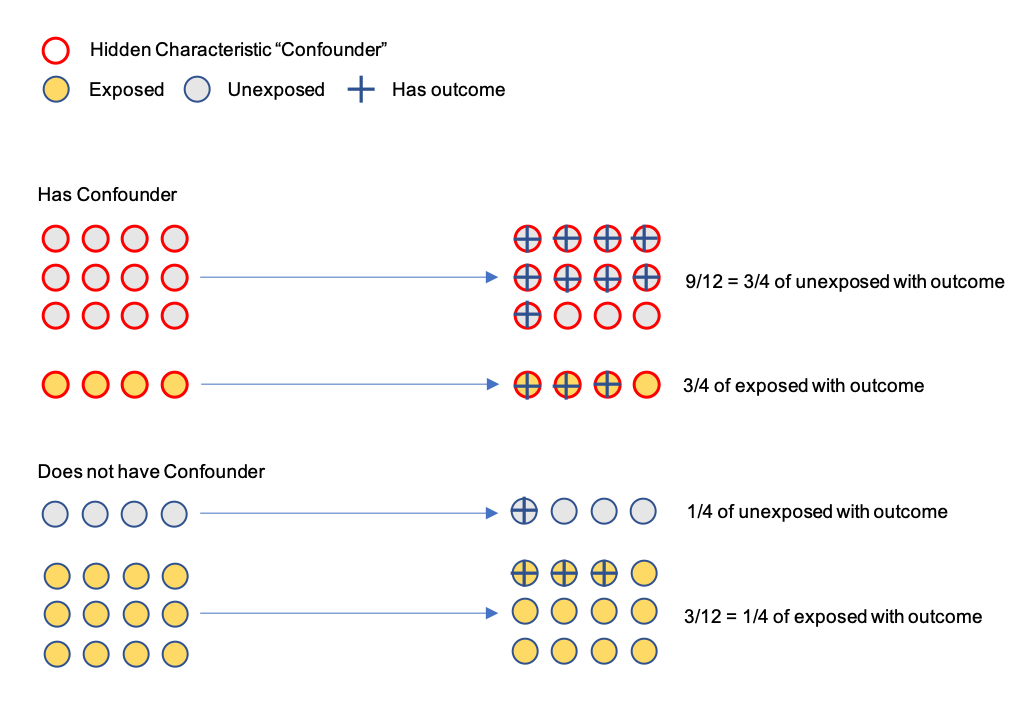
\includegraphics[width=0.9\textwidth,height=\textheight]{../media/confounder-3.png}

\end{frame}

\begin{frame}{Biases: Confounding and Stratification (5/5)}
\protect\hypertarget{biases-confounding-and-stratification-55}{}

If we have measured the confounder, then we can do what is called a
\textbf{stratified analysis}: look within the strata of the confounder
and assess the relationship between exposure and outcome separately.

You can see that within a given strata, the proportion who have the
outcome is identical among those exposed and unexposed. There is no
relationship between exposure and outcome.

Although we did this with a \textbf{binary} exposure and outcome,
similar techniques exist for a continuous exposure and outcome.

\end{frame}

\begin{frame}{Modeling: Intro}
\protect\hypertarget{modeling-intro}{}

The basic motivation behind statistical modeling in epidemiology is that
if you model the \emph{data generating process} with some unknown
parameters, then you can use observed data to estimate the unknown
parameters of the data generating process.

\[
Y = f(\theta)
\]

If we knew \(\theta\), then it might be interesting to generate some
\(Y\)'s. In fact, many mathematical modelers do this. But we are
interested in the \emph{inverse problem} -- given \(Y\), then what was
\(\theta\)?

\emph{The assumptions that you made in your study design go into
\(f(\theta)\)!}

\end{frame}

\begin{frame}{Modeling: Linear Models}
\protect\hypertarget{modeling-linear-models}{}

For most applications in epidemiology, the function \(f\) has some
additional data that has been collected on individuals. Quite often,
analyses use \emph{linear models}, and find the ``best fit'' to the
data.

\[
y = \alpha + \beta x
\]

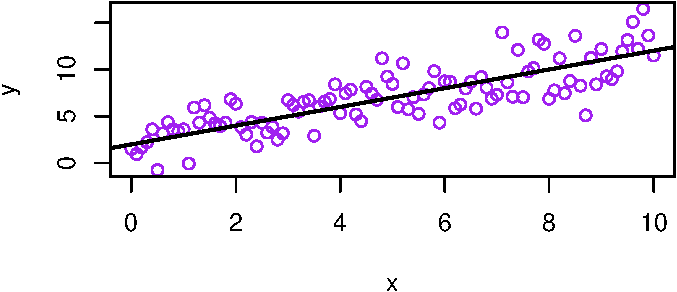
\includegraphics{biostats_I_files/figure-beamer/unnamed-chunk-1-1.pdf}

\end{frame}

\begin{frame}{Modeling: Generalized Linear Models}
\protect\hypertarget{modeling-generalized-linear-models}{}

If you have data that looks like the previous plot with a continuous
dependent variable, you're good to go with a basic linear regression.

Things get more complicated with different data types.

\[
g(y) = \alpha + \beta x
\]

\begin{table}[!h]

\caption{\label{tab:table2}Common Mean Relationships and Distributions in Epidemiology}
\centering
\fontsize{8}{10}\selectfont
\begin{tabular}{l|l|l|l|l}
\hline
\textbf{Data Type} & \textbf{Mean} & \textbf{Link Function} & \textbf{Statistical Distribution} & \textbf{Coefficients}\\
\hline
continuous & linear & g(y) = y & Gaussian & risk difference\\
\hline
counts & log-linear & g(y) = log(y) & Poisson & log risk ratio\\
\hline
binary & logistic-linear & g(y) = logit(y) & Bernoulli & log odds ratio\\
\hline
\end{tabular}
\end{table}

\end{frame}

\begin{frame}{Modeling: Randomized Controlled Trial}
\protect\hypertarget{modeling-randomized-controlled-trial}{}

Consider a \textbf{randomized controlled trial}. We have an independent
variable \(X\) that is \(1\) when the participant was randomized to
treatment and \(0\) when they received placebo. The outcome \(Y\) is
continuous. We could ask,

\begin{itemize}
\tightlist
\item
  What is the mean \(Y\) in the control group (\(x = 0\))?
\item
  What is the mean \(Y\) in the treatment group (\(x = 1\))?
\item
  What is the \emph{difference} between the mean outcome \(Y\) in
  treatment compared to control?
\end{itemize}

\end{frame}

\begin{frame}{Modeling: Linear Models}
\protect\hypertarget{modeling-linear-models-1}{}

Thinking about both the \textbf{data generating process} and the
\textbf{hypothesis that we want to answer}, we can parametrize a model.
\[
Mean[Y|X=x] = \alpha + \beta x
\]

\begin{itemize}
\tightlist
\item
  What is mean \(Y\) among controls (\(x = 0\))? \(\to \alpha\)
\item
  What is mean \(Y\) among treated (\(x = 1\))? \(\to \alpha + \beta\)
\item
  What is \emph{difference} between the mean outcome \(Y\) in treatment
  compared to control? \(\to \beta\)
\end{itemize}

\end{frame}

\begin{frame}{Modeling: Visualization}
\protect\hypertarget{modeling-visualization}{}

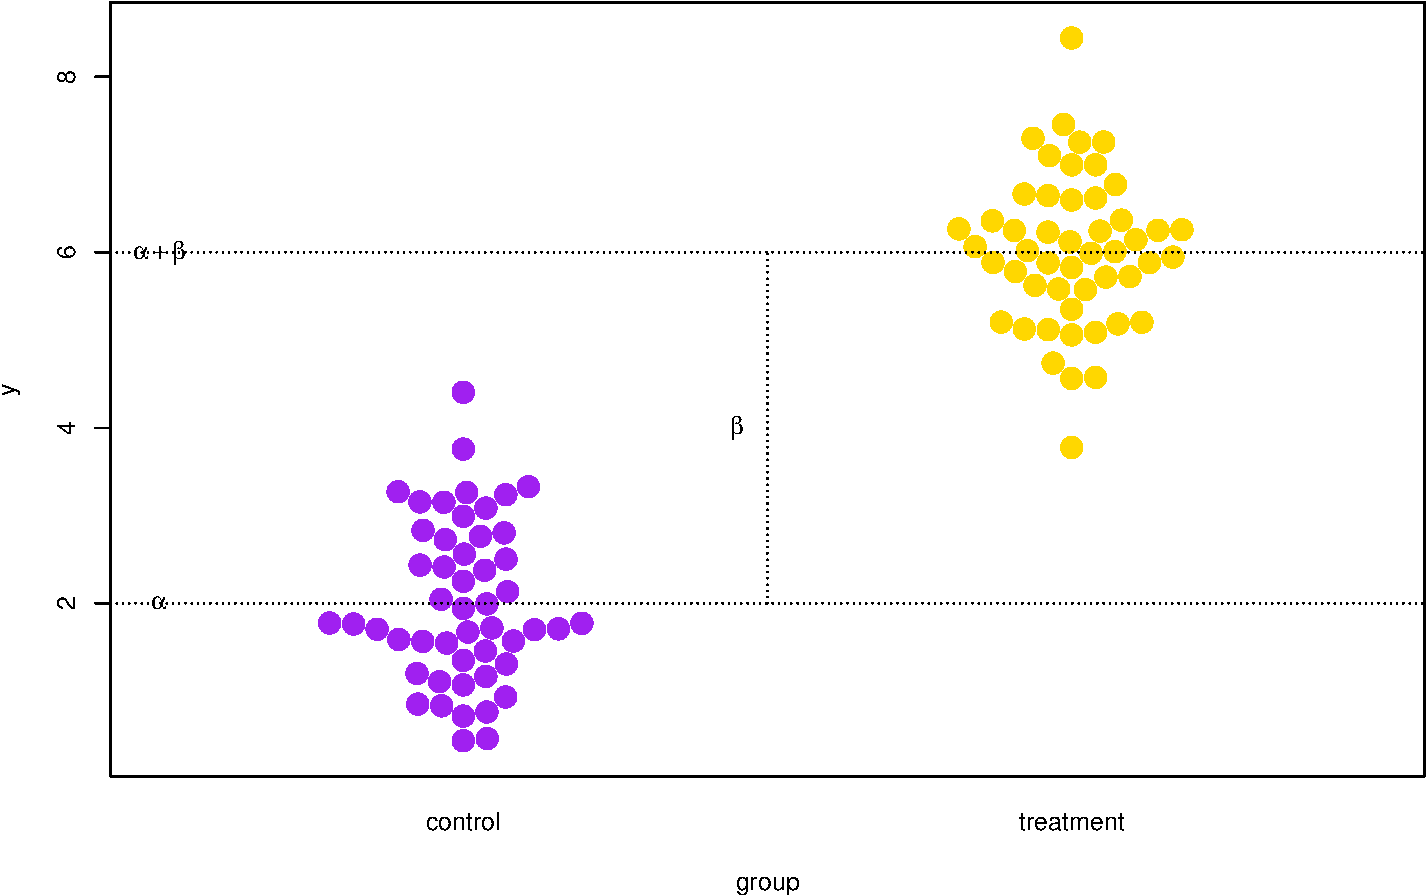
\includegraphics{biostats_I_files/figure-beamer/unnamed-chunk-2-1.pdf}

\end{frame}

\begin{frame}{Modeling: Example}
\protect\hypertarget{modeling-example}{}

Think back to our randomized controlled trial for women that have had a
stroke, and let \(Y\) be whether or not they died, and \(X\) be their
treatment group. We might start with the same linear model:

\[
Mean[Y|X] = \alpha + \beta X
\]

Do you see any problems with how this model is parametrized?

\end{frame}

\begin{frame}{Modeling: Example}
\protect\hypertarget{modeling-example-1}{}

Think back to our randomized controlled trial for women that have had a
stroke, and let \(Y\) be whether or not they died, and \(X\) be their
treatment group. We might start with the same linear model:

\[
Mean[Y|X] = \alpha + \beta X
\] Do you see any problems with how this model is parametrized?
\textbf{Yes! The mean can go beyond the {[}0, 1{]} range, which doesn't
make sense for a proportion.}

\end{frame}

\begin{frame}{Modeling: Example}
\protect\hypertarget{modeling-example-2}{}

From our example, it makes most sense to think of \(Y\) as a flip of a
loaded coin -- this is the Bernoulli distribution -- and how loaded the
coin is depends on the group \(X\).

\[
logit(Mean[Y|X]) = \alpha + \beta X \to Mean[Y|X] = \frac{e^{\alpha + \beta X}}{1 + e^{\alpha + \beta X}}
\]

This is called \emph{logistic regression}. Now \(\alpha + \beta x\)
explicitly modify the probability of having the outcome \(Y\), and it
must stay between 0 and 1.

\end{frame}

\begin{frame}{Modeling: Notes}
\protect\hypertarget{modeling-notes}{}

\begin{itemize}
\tightlist
\item
  I've only presented examples where the independent variables (or
  ``covariates'') are binary 0/1. The same methods can be used when the
  independent variable is continuous.
\item
  What I've presented so far is considered \emph{parametric} modeling,
  and it is common in epidemiology. You may come across \emph{semi-} or
  \emph{non-parametric} modeling as you're reading literature. It is a
  way to make fewer assumptions about the data generating process, but
  will typically come with the tradeoff of increased variability in the
  result.
\end{itemize}

\end{frame}

\begin{frame}{Inference}
\protect\hypertarget{inference}{}

How do we actually estimate \(\theta\) in \(Y = f(\theta)\)? There are a
variety of techniques depending on what \(f\) is, but one thing is for
certain -- \textbf{there will always be uncertainty}.

Inference is about making our \textbf{best guess} about \(\theta\), and
providing some degree of \textbf{confidence} in that guess (typically
95\% confidence). This may also include a \textbf{p-value} for a
hypothesis test.

Let's walk into these three elements in more detail -- (1) point
estimates, (2) confidence intervals, and (3) p-values.

\end{frame}

\begin{frame}{Inference: Point Estimates}
\protect\hypertarget{inference-point-estimates}{}

In order to make the ``best guess'' for the parameter we use information
about the distribution that is specified (e.g.~normal distribution) and
combine all of the observations together to figure out what value of
\(\theta\) is the \textbf{most likely}.

The \textbf{most likely} value is reported as the \textbf{point
estimate}.

\emph{``We estimate a risk ratio of \textbf{1.10}, meaning that there
was a 10\% increased risk of having the outcome in the exposed group
compared to controls.''}

\end{frame}

\begin{frame}{Inference: Confidence Intervals}
\protect\hypertarget{inference-confidence-intervals}{}

Confidence intervals (typically 95\%) represent the degree of
uncertainty that we have in our point estimate.

The interpretation is a bit counter-intuitive: if this experiment were
to be replicated 100 times, 95 of the confidence intervals constructed
in these experiments would cover the \textbf{true parameter}.

\emph{``We estimate a risk ratio of \textbf{1.10 (1.05 - 1.15)}, meaning
that there was a 10\% (5\% - 15\%) increased risk of having the outcome
in the exposed group compared to controls.''}

\end{frame}

\begin{frame}{Inference: P-Values}
\protect\hypertarget{inference-p-values}{}

If we have some estimate of \(\theta\), \(\hat{\theta}\), p-values make
sense in the context of a \textbf{hypothesis test}. It might look
something like this:

\[
H_0: \theta = 0 \quad H_1: \theta \neq 0
\]

This means: my \textbf{null} hypothesis is that \(\theta = 0\). In
linear regression, if \(\theta\) was the slope of the line, that means
\emph{there is no slope} (or no association).

A \textbf{p-value} of 0.05 has the following interpretation: the chance
of seeing a result this extreme or more extreme \textbf{if the null
hypothesis were true} is 5\%.

\emph{``We estimate a risk ratio of \textbf{1.10} with a p-value of
0.02. If there were truly no increased risk, there is a 2\% chance we
would see a result this extreme or more extreme.''}

\end{frame}

\begin{frame}{Inference: Simple Means}
\protect\hypertarget{inference-simple-means}{}

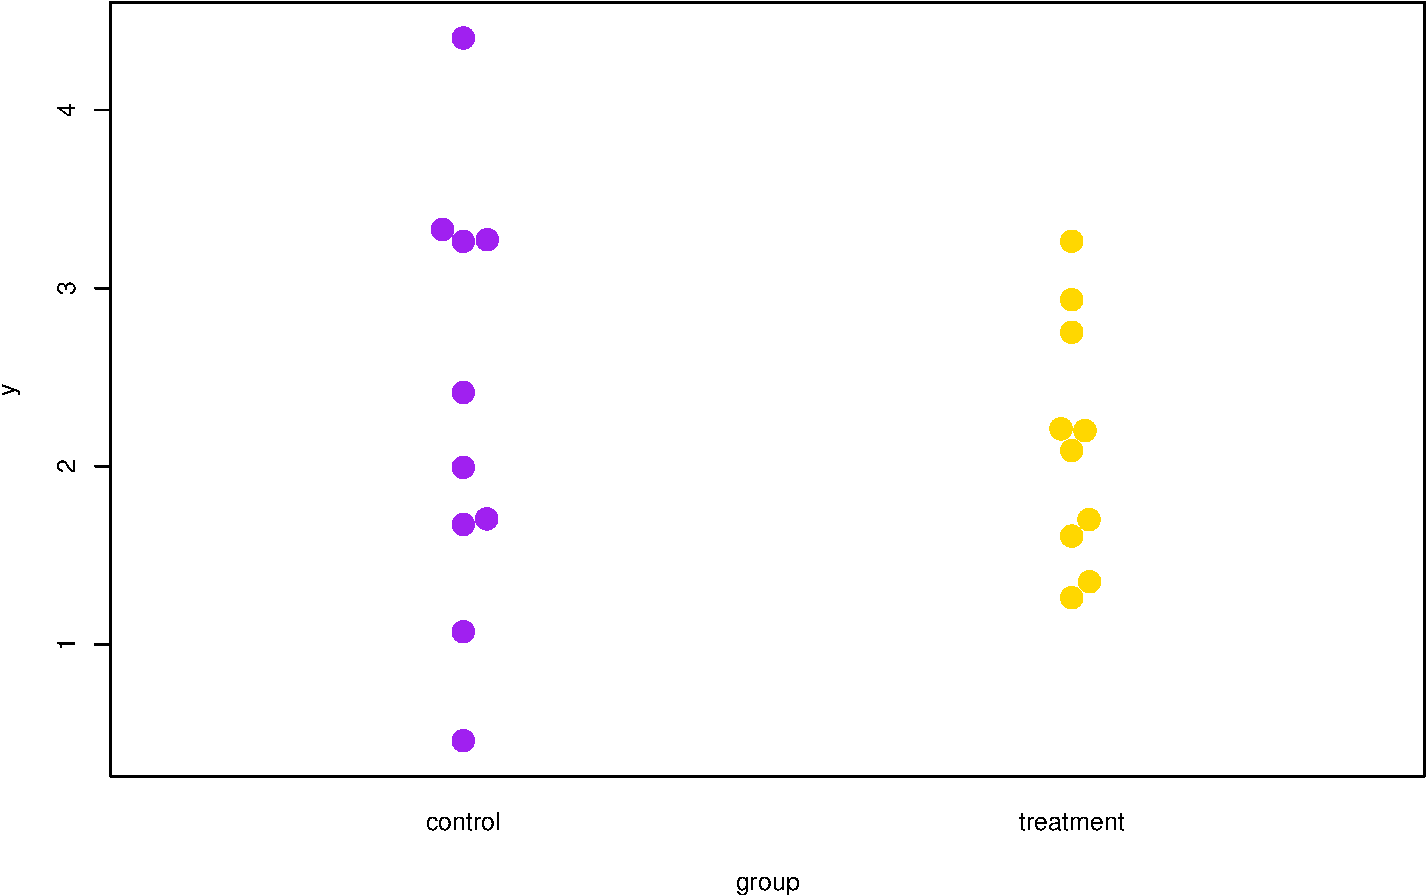
\includegraphics{biostats_I_files/figure-beamer/unnamed-chunk-3-1.pdf}

\end{frame}

\begin{frame}{Inference: Simple Means}
\protect\hypertarget{inference-simple-means-1}{}

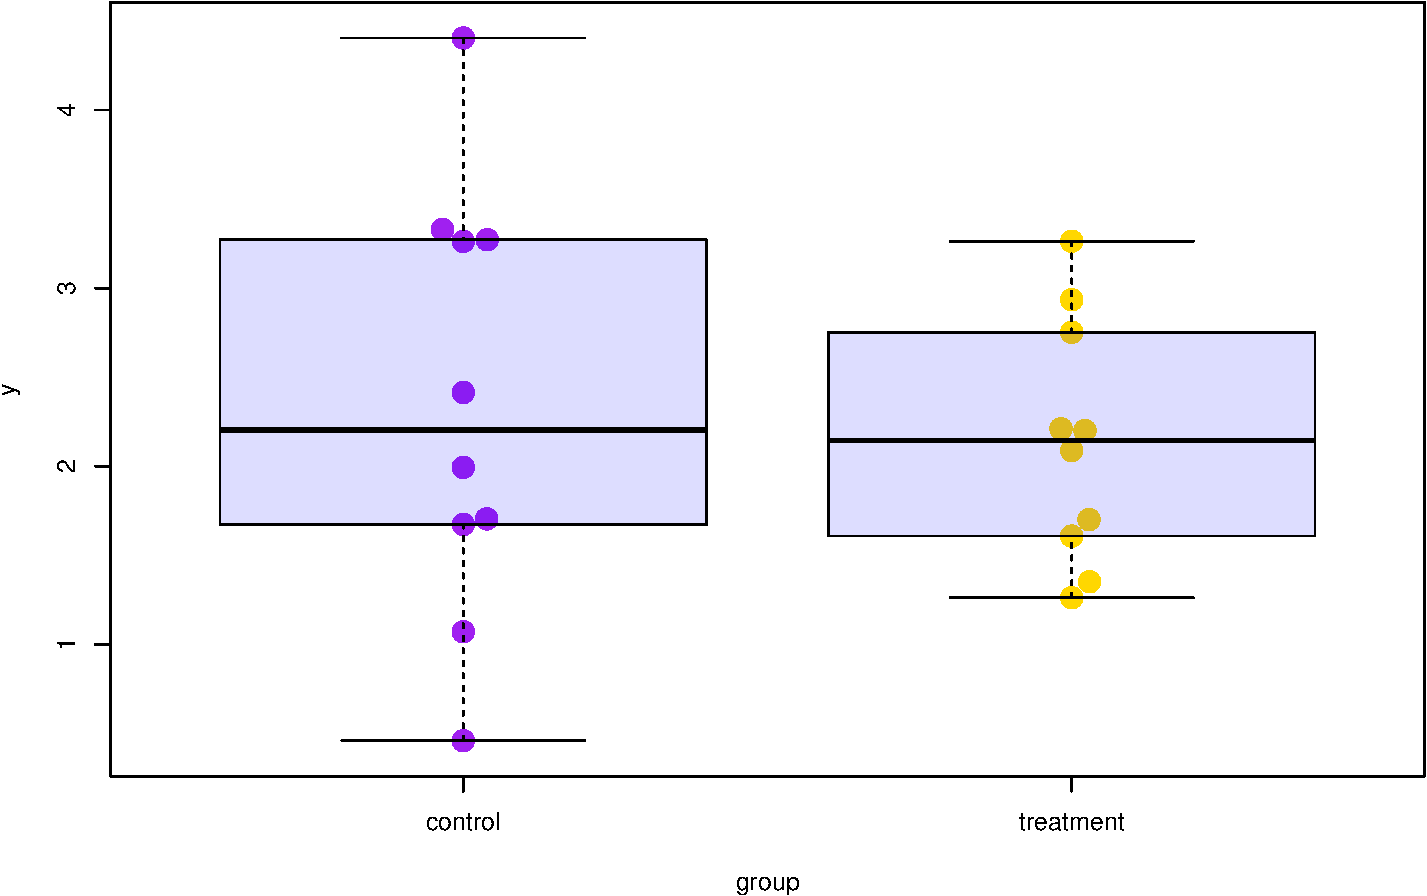
\includegraphics{biostats_I_files/figure-beamer/unnamed-chunk-4-1.pdf}

\end{frame}

\begin{frame}{Inference: Small Effect Size, Small Sample Size}
\protect\hypertarget{inference-small-effect-size-small-sample-size}{}

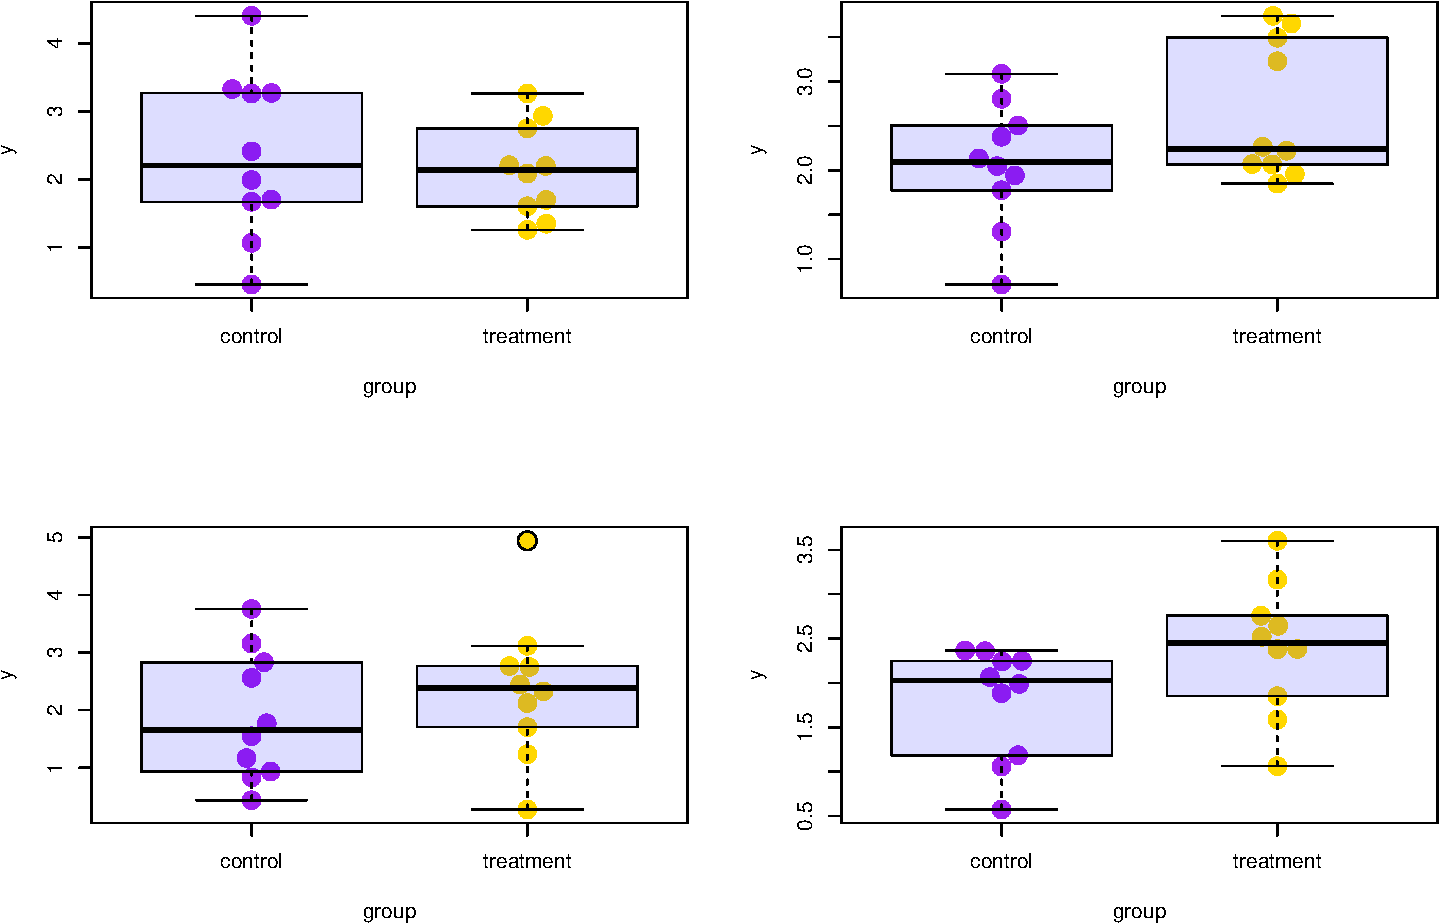
\includegraphics{biostats_I_files/figure-beamer/unnamed-chunk-5-1.pdf}

\end{frame}

\begin{frame}{Inference: Large Effect Size, Small Sample Size}
\protect\hypertarget{inference-large-effect-size-small-sample-size}{}

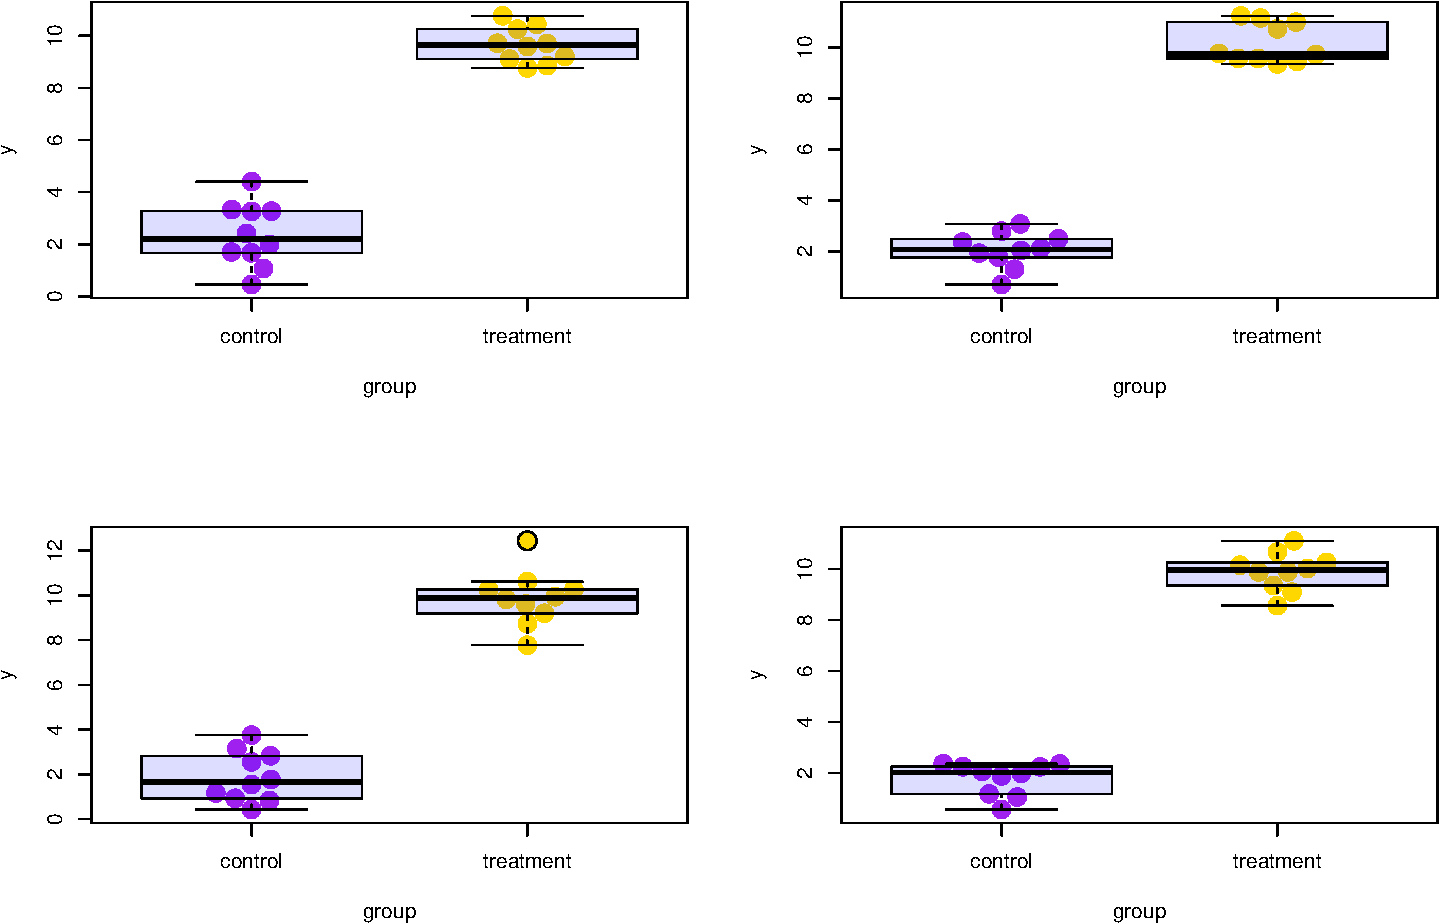
\includegraphics{biostats_I_files/figure-beamer/unnamed-chunk-6-1.pdf}

\end{frame}

\begin{frame}{Inference: Small Effect Size, Large Sample Size}
\protect\hypertarget{inference-small-effect-size-large-sample-size}{}

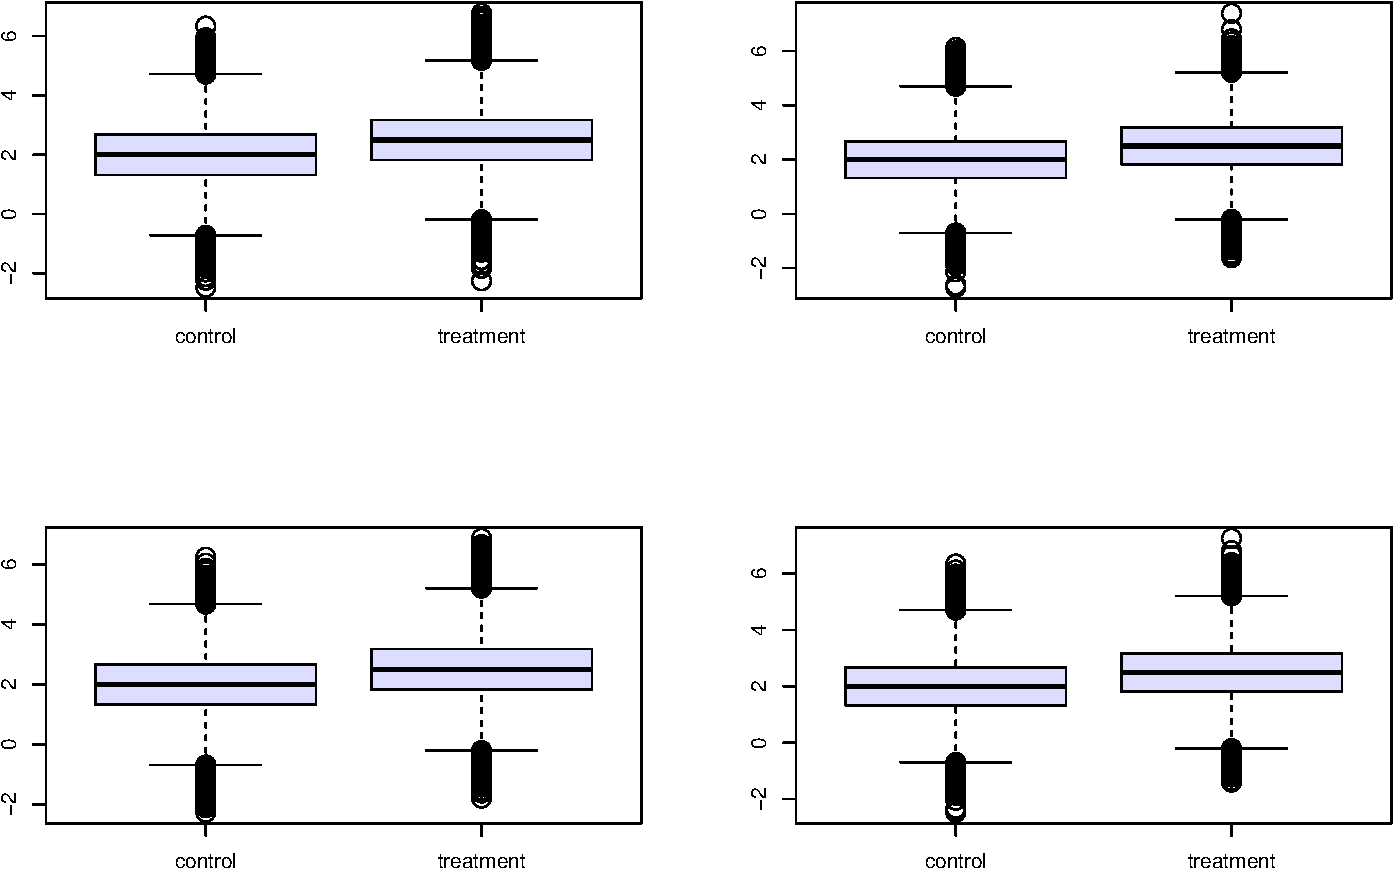
\includegraphics{biostats_I_files/figure-beamer/unnamed-chunk-7-1.pdf}

\end{frame}

\end{document}
